\documentclass{beamer}
\usepackage{beamerthemeAmsterdam}
\usepackage{amsmath}
\usepackage{graphicx}

\renewcommand{\phi}{\varphi}

\title{JPEG-2000}
\subtitle{De Wondere Wereld van Wavelets}
\author{Jan Westerdiep \and Okke van Garderen}
\date{\today}
\institute{Universiteit van Amsterdam}

\renewcommand{\itemize}[1]{\begin{itemize} #1 \end{itemize}}
\renewcommand{\figurename}{}

\begin{document}

\frame{\titlepage}

\section{Intro}

\frame{
  \frametitle{Recap}
  \begin{itemize}
  \item Project bij Rob Stevenson
  \item Originele JPEG $\implies$ Fouriertransformatie
  \item JPEG-2000 $\implies$ Wavelets
  \item Discreet signaal?
  \end{itemize}
}

\frame{
  \frametitle{Fouriertransformatie}
  \begin{columns}
    \begin{column}{0.75\linewidth}
      \[ \left\{ \phi_k(x) = e^{i k 2 \pi x}: k \in \mathbb{N}_0 \right\} \]
      \[ f = \sum \langle f, \phi_k \rangle \phi_k\text{, met $\phi_k$ genormaliseerd } \]

      \begin{itemize}
      \item Functie schrijven in de Fourierbasis
      \item Co\"effici\"enten kleiner dan $\epsilon$ ``weggooien"
      \item Signaal reconstrueren adhv kleinere set co\"effici\"enten
      \end{itemize}
    \end{column}
    \begin{column}{0.25\linewidth}
      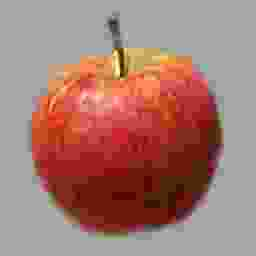
\includegraphics[width=\linewidth]{Sample2.jpg}
    \end{column}
  \end{columns}
}

\section{Wavelets}

\frame{
  \frametitle{Wavelettransformatie}
  \begin{columns}
    \begin{column}{0.4\linewidth}
      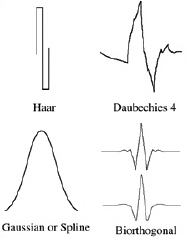
\includegraphics[width=\linewidth]{4wavelets.jpg}
    \end{column}
    \begin{column}{0.6\linewidth}
      \begin{itemize}
      \item Weer othonormale basis
      \item Kleinere drager $\implies$ discontinuiteiten alleen locaal zichtbaar
      \item Vari\"eteit aan families en klassen
      \item Schalingsfunctie $\phi$ en Waveletfunctie $\psi$
      \item JPEG-2000
      \end{itemize}
    \end{column}
  \end{columns}
}

\frame{
  \frametitle{Discrete Wavelettransformatie}
  \begin{columns}
    \begin{column}{0.6\linewidth}
      \begin{itemize}
      \item Op zoek naar $a_\lambda = \langle f, \phi_\lambda \rangle$
      \item Mallat: algoritme voor approximatie van functie
      \item Recursieve relaties: 
		\[\phi(x) = \textstyle\sum_k h_k \phi(2x-k)\]
		\[\psi(x) = \textstyle\sum_k g_k \phi(2x-k)\]
      \end{itemize}
\bigskip
      Mallat:
      \begin{eqnarray*}
        a_{i+1}[n] = \textstyle\sum_k h[k-2n]a_j[k] \\
        d_{i+1}[n] = \textstyle\sum_k g[k-2n]a_j[k]
      \end{eqnarray*}
    \end{column}
    \begin{column}{0.4\linewidth}
	\centering{Haar:}\\
	~\\
      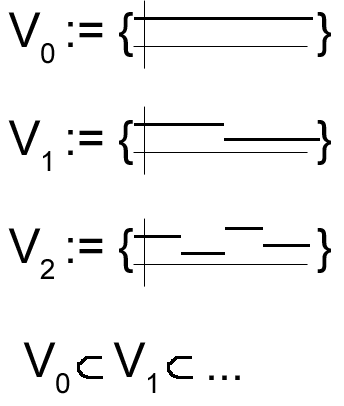
\includegraphics[width=\linewidth]{V_0V_1.png}
    \end{column}
  \end{columns}
}

\frame{
  \frametitle{Schema van Algoritme}
  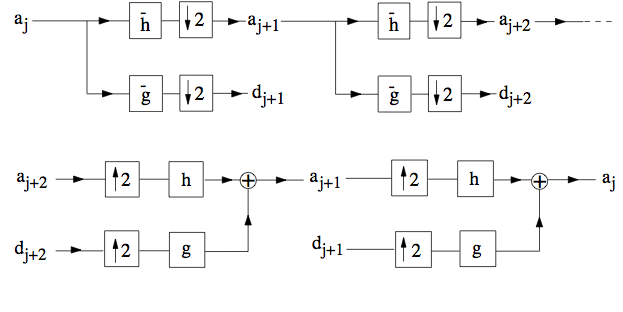
\includegraphics[width=\linewidth]{mallat.png}
}

\frame{
  \frametitle{Voorbeeld met Haar}
  \begin{columns}
    \vspace{-20pt} 
    \begin{column}{0.5\linewidth}
      \vspace{-20pt}
      
      De Haarwavelet heeft filters:
      \begin{itemize}
      \item $h = \frac 1 2 \sqrt 2 \cdot (-1,1)$
      \item $g = \frac 1 2 \sqrt 2 \cdot (1,1)$
      \end{itemize}
\bigskip
      Signaal : $a_0 = (1,2,1,2,3,4,3,4)$ \\

      $a_1 = \frac 1 2 \sqrt 2 \cdot (3,3,7,7)$\\
      $d_1 = \frac 1 2 \sqrt 2 \cdot (-1,-1,-1,-1)$\\

      $a_2 = (3,7)$\\
      $d_2 = (0,0)$\\

      $a_3 = \frac12\sqrt2\cdot (10)$\\
      $d_3 = \frac12\sqrt2\cdot (-4)$
    \end{column}
    \begin{column}{0.6\linewidth}
      \centering
      \begin{columns}
        \begin{column}{0.4\linewidth}
          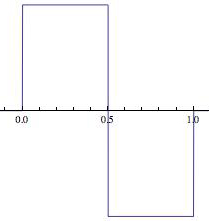
\includegraphics[width=\linewidth]{HaarWavelet_Psi.jpg}
        \end{column}
        \begin{column}{0.4\linewidth}
          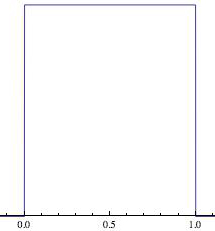
\includegraphics[width=\linewidth]{HaarWavelet_Phi.jpg}
        \end{column}
      \end{columns}
      \begin{eqnarray*}
        a_{i+1}[n] = \sum_k h[k-2n]a_i[k] \\
        d_{i+1}[n] = \sum_k g[k-2n]a_i[k]
      \end{eqnarray*}
      
  Uiteindelijk getransformeerde wordt:
  $\frac12\sqrt2\cdot(10,-4,0,0,-1,-1,-1,-1)$

    \end{column}
  \end{columns}
}

\frame{
  \frametitle{Daubechies 4 (ook wel Daubechies 2)}
  \begin{columns}
    \begin{column}{0.5\linewidth}
      \begin{itemize}
        \item Grotere drager $\implies$ slechter met discontinuiteiten
        \item Langere filter
        \item Gaat beter om met locale gladheid
        \item Subjectief: minder hoekig beeld
      \end{itemize}
    \end{column}
    \begin{column}{0.5\linewidth}
      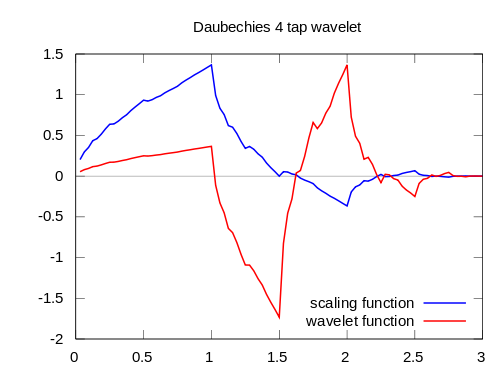
\includegraphics[width=0.8\linewidth]{daubechies.png}
    \end{column}
  \end{columns}
}

\section{Plaatjes}

\frame{
  \frametitle{2-dimensionaal signaal (Plaatjes)}
\begin{columns}
  \begin{column}{0.6\linewidth}
    \begin{itemize}
    \item E\'en approximatiekwadrant en drie detailkwadranten
    \item Tweedimensionale functies maken:
      \[\begin{array}{c|c}
        \phi \otimes \phi & \psi \otimes \phi \\\hline
        \phi \otimes \psi & \psi \otimes \psi
      \end{array}\]
    \item Generalisatie naar meer dimensies
    \end{itemize}
  \end{column}
  \begin{column}{0.5\linewidth}
    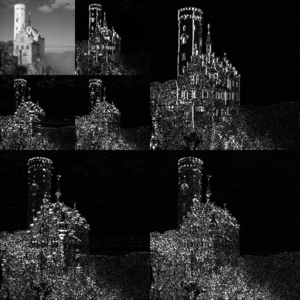
\includegraphics[width=\linewidth]{mallat-schema.png}
  \end{column}
\end{columns}
}

\frame{
  \frametitle{Voorbeelden (20\%)}
  \begin{table}
    \begin{tabular}{ c c }
      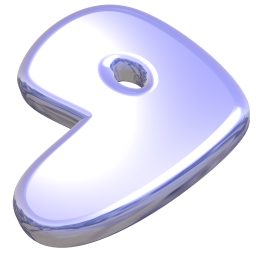
\includegraphics[width=0.3\linewidth]{gentoo.png} &
      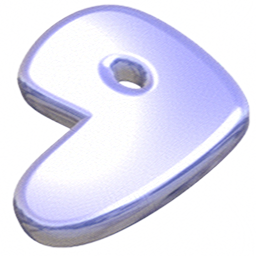
\includegraphics[width=0.3\linewidth]{gentoo_new_20p.png} \\

      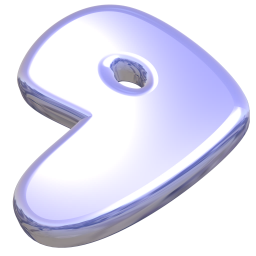
\includegraphics[width=0.3\linewidth]{gentoo_20_haar.png} &
      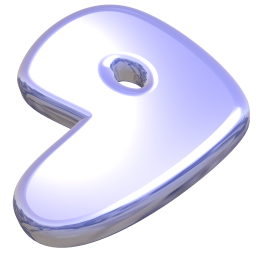
\includegraphics[width=0.3\linewidth]{gentoo_20_db2.png} 
    \end{tabular}
  \end{table}
}

\frame{
  \frametitle{Voorbeelden (8\%)}
  \begin{table}
    \begin{tabular}{ c c }
      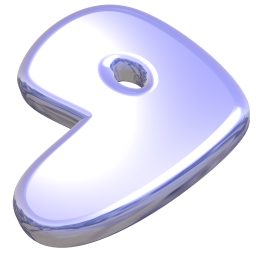
\includegraphics[width=0.3\linewidth]{gentoo.png} &
      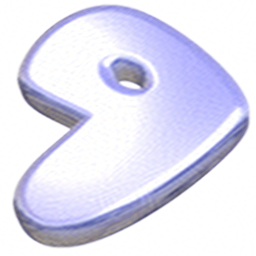
\includegraphics[width=0.3\linewidth]{gentoo_new_8p.png} \\

      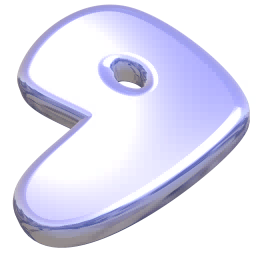
\includegraphics[width=0.3\linewidth]{gentoo_08_haar.png} &
      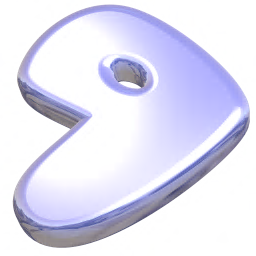
\includegraphics[width=0.3\linewidth]{gentoo_08_db2.png} 
    \end{tabular}
  \end{table}
}

\frame{
  \frametitle{Voorbeelden (1\%)}
  \begin{table}
    \begin{tabular}{ c c }
      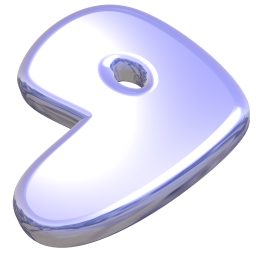
\includegraphics[width=0.3\linewidth]{gentoo.png} &
      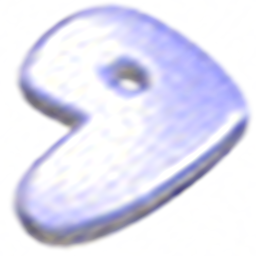
\includegraphics[width=0.3\linewidth]{gentoo_new_1p.png} \\

      
\includegraphics[width=0.3\linewidth]{gentoo_01_haar_smooth.png} &
      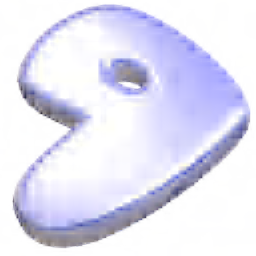
\includegraphics[width=0.3\linewidth]{gentoo_01_db2_smooth.png} 
    \end{tabular}
  \end{table}
}

\section{Filmpjes}

\frame{
  \frametitle{Filmpjes $\implies$ 3D signaal}
  \begin{itemize}
  \item Natuurlijke voortzetting van Mallatdecompositie
  \item Opeenvolgende frames opvatten als 3e dimensie
  \end{itemize}
}

\frame{
  \frametitle{Maar toen...}
  \begin{itemize}
  \item Vermoeden van Rob over filmpjes
  \item Tensorproduct i.p.v. Mallatdecompositie
  \item Potentieel beter bij weinig dicontinuiteiten
  \end{itemize}
  \centering
  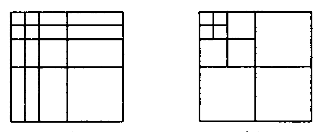
\includegraphics[width=0.5\linewidth]{mallat-vs-tensor.png} 
}

\section{Wat nu?}

\frame{
  \frametitle{Inhoudsopgave}
  \begin{itemize}

  \item Deel over Fourier

    \begin{itemize}
    \item[-] Analyse van Discrete Fourier Transform
    \item[-] Fast Fourier Transform-algoritme
    \item[-] Toepassing van FFT op plaatjes/geluid
    \end{itemize}

  \item Deel over Wavelets

    \begin{itemize}
    \item[-] Theoretische beschouwing van wavelets
    \item[-] Toepassing van Wavelets $\implies$ DWT
    \item[-] Analyse van de DWT
    \item[-] Toepassing van DWT op plaatjes/geluid
    \item[-] Tensorproduct en filmpjes
    \end{itemize}

  \item Vergelijkend deel Wavelets vs. Fourier en Resultaten
  \end{itemize}
}

\frame{
  \frametitle{Wat nog moet gebeuren}
  \begin{itemize}
  \item Kijken naar convergentie-eigenschappen van de fout (hoe goed is de benadering theoretisch)
  \item Afronden van wat we nu hebben
  \item Eventueel nog iets interessants onderzoeken
  \item Code opschonen
  \end{itemize}
}

\frame{
   Recursieve relatie door geneste ruimtes:
   \bigskip

   Laat $V_i = span\{\phi_{i,n} : n \in \mathbb{Z}\},\quad W_i = span\{\psi_{i,n}:n \in \mathbb{Z}\}$

   $V_{i+1} = V_i \oplus W_i \implies V_n = V_0 \oplus W_0 \oplus \ldots \oplus W_{n-1}$
   \bigskip

   Dus $\phi_i$ en $\psi_i$ te schrijven zijn in termen van $\phi_{i+1}$.\\
   Ook $\psi_i$ zijn een basis voor $V_n$
}

\end{document}
